\section{Probabilistic Modal Logic}
\label{sec:pml}

\subsection{Syntax and Semantics}

In this section we present some preliminary notions over probabilistic logics. 
In what follows, let $\prop$ be a non-empty countable set of atomic propositions. Also, for every relation $E\subseteq S\times S$, we use the abbreviation:
\[ 
    E[U]=\{v \in S  \mid (u,v)\in E \text{ for some }u\in U \}. 
\] 

\begin{definition} A \emph{probabilistic Kripke model} is a tuple $\M=(W,P, V)$ where:

\begin{itemize}
    \item $W$ is a countable set of states or worlds; 
    \item $P : W \times W \rightarrow [0,1]$ is the transition probability matrix where for all $w \in W$, $\displaystyle\sum_{w' \in W} P(w, w') = 1$;
    \item $V : \prop \rightarrow 2^W$ is a function that assigns to each $p \in \prop$ the set of states in which $p$ holds.
\end{itemize}
\end{definition}

%An execution of PTS \( D = (S,  P, L) \) is represented by a path. Formally, a path \( \omega \) is a non-empty sequence of states \( s_0 s_1 s_2 \dots \) in $S$ where\( P(s_i, s_{i+1}) > 0 \) for all \( i \geq 0 \).


%%% comented text %%%%%
%A path can be either finite or infinite. We denote by \( \omega(i) \) the \( i \)-th state of a path \( \omega \), \( |\omega| \) the length of \( \omega \) (number of transitions), and for a finite path \( \omega_{\text{fin}} \), the last state by \( \text{last}(\omega_{\text{fin}}) \). We say that a finite path \( \omega_{\text{fin}} \) of length \( n \) is a prefix of the infinite path \( \omega \) if \( \omega_{\text{fin}}(i) = \omega(i) \) for \( 0 \leq i \leq n \). The sets of all infinite and finite paths of \( D \) starting in state \( s \) are denoted \( \text{Path}_D(s) \) and \( \text{Path}_D^{\text{fin}}(s) \), respectively. Unless stated explicitly, we always deal with infinite paths.

%In order to reason about the probabilistic behaviour of the DTMC, we need to determine the probability that certain paths are taken. This is achieved by defining, for each state \( s \in S \), a probability measure \( \text{Pr}_s \) over the set of infinite paths \( \text{Path}_D(s) \).\\
%(We should put references how to define such probability measure)

%Below, we give an outline of this construction. For further details, see [41]. The probability measure is induced by the transition probability matrix \( P \) as follows. For any finite path \( \omega_{\text{fin}} \in \text{Path}_D^{\text{fin}}(s) \), we define the probability \( \text{P}_s(\omega_{\text{fin}}) \):
%$$ \text{P}_s(\omega_{\text{fin}}) \triangleq 
%\begin{cases} 
%1 & \text{if } n = 0, \\
%P(\omega(0), \omega(1)) \cdot \dots \cdot P(\omega(n-1), \omega(n)) & \text{otherwise},
%\end{cases}
%$$
%where \( n = |\omega_{\text{fin}}| \). Next, we define the cylinder set \( C(\omega_{\text{fin}}) \subseteq \text{Path}_D(s) \) as:
%$$
%C(\omega_{\text{fin}}) \triangleq \{ \omega \in \text{Path}_D(s) \mid \omega_{\text{fin}} \text{ is a prefix of } \omega \}.
%$$


%\subsection{Probabilistic Computation Tree Logic (PCTL)}

%Specifications for DTMC models can be written in PCTL (Probabilistic Computation Tree Logic)~\cite{baier2008}, a probabilistic extension of the temporal logic CTL (put a reference for it).

%\begin{definition}[\cite{Kwiatkowska2007}] The grammar of PCTL is the  following

%\[
%\Phi ::= \textbf{true} \mid a \mid \neg \Phi \mid \Phi \land \Phi \mid \mathbb{P}_{\sim p}[\phi]
%\]
%\[
%\phi ::= \textsf{X} \, \Phi \mid \Phi \, \mathsf{U}^{\leq k} \Phi
%\]

%\noindent\textit{where $a$ is an atomic proposition, $\sim \in \{<, \leq, \geq, >\}$, $p \in [0,1]$ and $k \in \mathbb{N} \cup \{\infty\}$.}
%\end{definition}




%\begin{definition} Let \( \M = (S, P, L) \) be PTS. For any state \( s \in S \), the satisfaction relation \( \models \) is defined by:
%\begin{itemize}
%\item$
%\M,s \models \text{true} \quad \text{for all } s \in S
%$\item $
%\M,s \models a \iff a \in L(s)
%$\item $
%\M,s \models \neg \Phi \iff s \not\models \Phi
%$\item $
%\M,s \models \Phi \land \Psi \iff s \models \Phi \land s \models \Psi
%$\item $
%\M, s \models P \sim p[\phi] \iff \text{Prob}_\M(s, \phi) \sim p
%$\\ \textcolor{red}{$\M, s \models P \sim p[\textsf{X}^a\Phi] \iff \text{Prob}_\M(s, \textsf{X} \Phi,a) \sim p$}
%\item \textcolor{red}{$\M, s \models P \sim p[\phi \, U_k \Psi] \iff \text{Prob}_\M(s, \textsf{X} \Phi,0) \sim p$}
%\end{itemize}
%where:

%$\text{Prob}_\M(s, \phi) := \Pr_s \{ \omega \in \text{Path}_\M(s) \mid \M,\omega \models \phi \}$

%and for any path \( \omega \in \text{Path}_\M(s) \):

%\medskip


%$\M,\omega \models X \Phi \iff \omega(1) \models \Phi$

%$\M,\omega \models \phi \, U_k \Psi \iff \exists i \in \mathbb{N} \, ( i \leq k \land \M,\omega(i) \models \Psi \land \forall j < i \, (\omega(j) \models \Phi) )$

%\end{definition}


%Note that, for any state \( s \) and path formula \( \phi \), the set \( \{ \omega \in \text{Path}_D(s) \mid \omega \models \phi \} \) is a measurable set of \( (\text{Path}_D(s), \Sigma_{\text{Path}_D(s)}) \) and hence \( \Pr_s \) is well defined over this set. 

%\section{Dynamic PTS}

%When we are evaluating a $X \Phi$ formula in path $w$ of PTS we may change the model and then $we evaluate it in a different 

%\newpage
%\section{Another possibility} This was the original one.



% \subsection{Probabilistic modal logic} %(see this https://cdn.aaai.org/AAAI/2007/AAAI07-077.pdf)

We adopt the probabilistic definition of modal logic in~\cite{ALDINI2024109167}. Notice that the definition of truth is \emph{crisp}, i.e., it is either true or false.

\begin{definition}[Formulas] 
The set of formulas is defined recursively as:
\[
\varphi, \psi ::= p \mid \neg \varphi \mid \varphi \vee \psi \mid \Diamond_\rho \varphi,
\]
where $p\in\prop$ and $\rho \in [0,1]$. We assume other Boolean operators are defined in a usual way.
\end{definition}

\begin{definition}[Satisfaction]
Let $\M = (W, P, V)$ be a probabilistic Kripke structure, and let $w$ be a state in $W$. For any probabilistic modal logic formula~$\varphi$, we define 
the satisfaction relation $\models$ recursively as follows:
%$\operatorname{val}(s, \varphi)$ recursively as follows:

\[
\begin{array}{l@{\ \  }c@{\ \ }l}
\M,w \models p & \iff & w\in V(p) \\
\M,w \models \neg\varphi & \iff & \M,w\not\models\varphi \\
\M,w \models \varphi\vee\psi & \iff & \M,w\models\varphi \text{ or } \M,w\models\psi \\
\M,w \models \Diamond_\rho\varphi & \iff & \displaystyle\sum_{\{v\in W \ \mid \ \M,v\models\varphi\}} P(w, v) \ge \rho.
\end{array}
\]
\end{definition}

\medskip

\begin{example}\label{ex1}
To illustrate how the satisfaction is evaluated on a probabilistic Kripke model, consider the structure depicted in Fig. \ref{fig:classic}.

\begin{figure}[!ht]
    \centering
        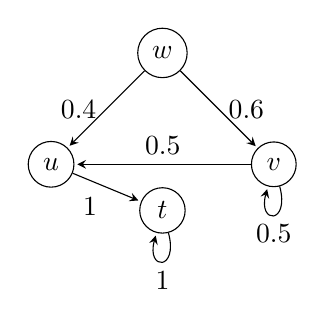
\begin{tikzpicture}[->,>=stealth,shorten >=1pt,auto,node distance=2cm]
        
        % Nodes
        \node[circle,draw] (w) {$w$};
        \node[circle,draw,below left of=w] (u) {$u$};
        \node[circle,draw,below right of=w] (v) {$v$};
        \node[circle,draw,below of=w] (t) {$t$};
        
        % Edges
        \path (w) edge node[left] {$0.4$} (u)
              (w) edge node[right] {$0.6$} (v)
              (u) edge node[below left] {$1$} (t)
              (v) edge node[above] {$0.5$} (u)
              (v) edge [loop below] node {$0.5$} (v)
              (t) edge [loop below] node {$1$} (t);
        
        \end{tikzpicture}
    \caption{Example of probabilistic Kripke model.}
    \label{fig:classic}
\end{figure}

Let $\prop=\{p,q\}$, we define a model $\model=(W,P,V)$ where  $W=\{u,v,w,t\}$, $P$ is the transition probability matrix depicted in Table~\ref{prob_matrix} and $V: \prop\rightarrow 2^W$ is defined such that $V(p)=\{u,w,t\}$ and $V(q)=\{v,t\}$.

\begin{table}[!ht]
    \centering
        \caption{Transition probability matrix of model depicted in Fig. \ref{fig:classic}.}
    \begin{tabular}{|c|c c c c|}
        \hline
         &$\quad u\quad$&$\quad v\quad$&$\quad w\quad$&$\quad t\quad$ \\\hline
         $\>u\>$&&&&1\\
         $v$&0.5 & 0.5&$\quad$&\\
         $w$& 0.4&0.6&&\\
         $t$& &&&1\\ \hline
    \end{tabular}
    \label{prob_matrix}
\end{table}

As an example, let us evaluate the formula $\Diamond_{0.5}(p \vee \Diamond_{0.8} \ q)$ at the state $w$:

\smallskip

$\M,w \models \Diamond_{0.5}(p \vee \Diamond_{0.8} \ q) \ \iff \ \displaystyle\sum_{\{x\in W \ \mid \ \M,x\models p \vee \Diamond_{0.8} \ q\}} P(w, x) \geq 0.5.$

Thus, for each state $x\in W$, we need to check whether $\model,x\models p \vee \Diamond_{0.8} \ q$, which holds if and only if $\model,x\models p$ or $\model,x\models \Diamond_{0.8} \ q$. Since $V(p)=\{u,w,t\}$, we only need to check the case $x=v$: 

$\model,v\models \Diamond_{0.8} \ q \ \iff \displaystyle\sum_{\{y \ \in W \ \mid \ \M,y\models \ q\}} P(v, y) \geq 0.8$.  According to the semantics, this is the case iff $P(v,v) + P(v,t) \geq 0.8$. But then we get $0.5 \geq 0.8$, which is false. \

Hence, $\displaystyle\sum_{\{x\in W \ \mid \ \M,x\models p \vee \Diamond_{0.8} \ q\}} P(w, x) \geq 0.5$ holds iff $P(w,w)+P(w,u) + P(w,t)\geq 0.5$, iff  $0.4 \geq 0.5$, which is false.

Therefore, $\M,w \not\models \Diamond_{0.5}(p \vee \Diamond_{0.8} \ q)$.

\end{example}


\subsection{Bisimulation}
%\textcolor{blue}{RF: the notions below are auto(bi)simulations. Is there a reason, or do we want it between two different models?}\textcolor{red}{It is not clear  how to define it. Here we have the condition of being a equivalence relation.} 
%\begin{definition}
%  Given a  probabilistic Kripke model  $\M=(S,P, V)$, a \emph{simulation} on $\M$ is an equivalence relation $B$ on $S$ such that it $s B s'$ we have
%  \begin{itemize}
%\item  $s\in V(p) $ iff $s'\in V(p) $
%\item for all $\displaystyle y\in S,  \sum_{w\in [y]} P(s,w) \leq\sum_{w\in [y]} P(s',w)$ %Find example of simulation that is not bisimulation
%\end{itemize}

%A bisimulation on $\M$ is an equivalence relation $B$ on $S$ such that it $s B s'$ we have
%\begin{itemize}
%\item  $s\in V(p) $ iff $s'\in V(p) $
%\item for all $\displaystyle y\in S,  \sum_{w\in [y]} P(s,w) =\sum_{w\in [y]} P(s',w)$
%\end{itemize}
%Being an equivalence relation can be dropped? 
  
%\end{definition}

%Two states are said to be probabilistically bisimilar if there is some such R relating them.

%\begin{theorem}
   % Given a  probabilistic Kripke model  $\M=(S,P, V)$ and  a \emph{simulation} on $\M$. Then for any $(w,w')\in B$ and any formula $\varphi$ we have $$\M,w \models \varphi \Longrightarrow \M,w' \models \varphi$$

%Moreover if  $B$ is a bisimulation we get  
    
 %$$\M,w \models \varphi \Longleftrightarrow \M,w' \models \varphi$$
    
%\end{theorem}

%NEW defintion

We now introduce a definition of bisimulation for the basic probabilistic case. While the classical definition usually defines bisimulation as an equivalence relation over the states of a probabilistic Kripke model, we introduce a version here to relate two different probabilistic Kripke models.

Probabilistic structures with labeled edges but without propositions are studied in~\cite{Panangaden2011}. In that paper, the author introduces the definition of dynamic relation based on the work in~\cite{BW01b,BW01a}, which does not require the relation to be an equivalence relation. Moreover, he proves that a dynamic relation implies the existence of a bisimulation relation. There, he was also able to prove the invariance and Hennessy-Milner theorem for finite models. Although that paper considers a probabilistic Kripke structure with labels, we use it as the basis for our definition within a context that also considers propositions.

\begin{definition}[Bisimulation]\label{bis} Let  $\M=(W,P, V)$ and  $\M' = (W', P', V')$ be two probabilistic Kripke models and $E \subseteq W \times W'$. We say that a nonempty relation $E$ is a \emph{bisimulation from $\M$ to $\M'$} if for every $w \in W$ and $w' \in W'$ such that $wEw'$, we have

\begin{description}
    \item[(atom):] for any $p \in \prop$, $w\in V(p)$ iff $w'\in V'(p)$,
    \item[(p-zigzag):] for any $U \subseteq W$, $\displaystyle \sum_{u \in U} P(w, u) \leq \displaystyle \sum_{u' \in E[U]} P'(w', u')$
\end{description}
\end{definition}

\begin{remark}
    Observe that the condition \textbf{(p-zigzag)} entails also its mirror condition \textbf{(p-zigzag')}. To prove this, let us consider a set $U'\subseteq W'$ and aiming for a contradiction assume that the following inequality holds:
    \begin{equation} \label{eq:zagzig}
        \displaystyle \sum_{u' \in U'} P'(w', u') > \displaystyle \sum_{ u  \in  E^{-1}[U']} P(w, u)
    \end{equation}
    We define $T := W \setminus E^{-1}[U']$ and observe that if $v'\in E[T]$ then $v'\notin U'$, so $U'$ and $E[T]$ are disjoint. 

    The condition \textbf{(p-zigzag)} for $T$ establishes that:
    \begin{equation} \label{eq:zigzag}
        \displaystyle \sum_{v \in T} P(w, v) \leq \displaystyle \sum_{ v' \in E[T]} P'(w', v')
    \end{equation}
    Now, combining equations \eqref{eq:zagzig} and \eqref{eq:zigzag} we get:
    \begin{multline}
        \label{eq:zagzig+zigzag}
        \displaystyle \sum_{v \in T} P(w, v) 
        +
        \displaystyle \sum_{ u \in E^{-1}[U']} P(w, u) <  
        \displaystyle \sum_{ v' \in E[T]} P'(w', v')
        +
        \displaystyle \sum_{u' \in U'} P'(w', u')
    \end{multline}
    Since $W = T \cup E^{-1} [U'] $, we have that:
    \begin{equation}
        \label{eq:first_part}
        \displaystyle \sum_{v \in T} P(w, v) 
        +
        \displaystyle \sum_{ u \in E^{-1}[U']} P(w, u)
        =
        1
    \end{equation}
    Based on the observation that $U'$ and $E[T]$ are disjoint, we can conclude that:
    \begin{equation}
        \label{eq:second_part}
        \displaystyle \sum_{ v' \in  E[T]} P'(w', v')
        +
        \displaystyle \sum_{u' \in U'} P'(w', u')
        \leq
        1
    \end{equation}
    Therefore, combining \eqref{eq:zagzig+zigzag}, \eqref{eq:first_part} and \eqref{eq:second_part} we get a contradiction.
\end{remark}

With this definition at hand, we are able to prove the following characterization result, usually called the \emph{invariance under bisimulation theorem}.

\begin{theorem}\label{th:inv_prob} Let  $\M=(W,P, V)$ and $\M' = (W', P', V')$ be two probabilistic Kripke models and $E \subseteq W \times W'$ a bisimulation from $\M$ to $\M'$. Then for any $(w,w')\in E$ and any formula $\varphi$ we have  $$\M,w \models \varphi \text{ iff } \M',w' \models \varphi$$
\end{theorem}

\begin{proof}
    The proof is obtained as a fragment of the proof of Theorem \ref{th:invariance}, that will be presented later on the paper.
\end{proof}